\documentclass{article}
%\usepackage[margin=1in]{geometry}
\setlength\topmargin{0pt}
\addtolength\topmargin{-\headheight}
\addtolength\topmargin{-\headsep}
\setlength\oddsidemargin{0pt}
\setlength\textwidth{\paperwidth}
\addtolength\textwidth{-2in}
\setlength\textheight{\paperheight}
\addtolength\textheight{-2in}

\usepackage[english]{babel}
\usepackage[utf8]{inputenc}
\usepackage{fancyhdr}
\usepackage{listings}
\usepackage{graphicx}
\usepackage{xcolor}
\usepackage{amsmath}


\definecolor{codegreen}{rgb}{0,0.6,0}
\definecolor{codegray}{rgb}{0.5,0.5,0.5}
\definecolor{codepurple}{rgb}{0.58,0,0.82}
\definecolor{backcolour}{rgb}{0.95,0.95,0.92}


\usepackage{booktabs}
\usepackage{pgfplotstable}



\lstdefinestyle{mystyle}{
	backgroundcolor=\color{backcolour},
	commentstyle=\color{codegreen},
	keywordstyle=\color{magenta},
	numberstyle=\tiny\color{codegray},
	stringstyle=\color{codepurple},
	basicstyle=\ttfamily\footnotesize,
	breakatwhitespace=false,
	breaklines=true,
	captionpos=b,
	keepspaces=true,
	numbers=left,
	numbersep=5pt,
	showspaces=false,
	showstringspaces=false,
	showtabs=false,
	tabsize=2
}
\lstset{style=mystyle}

\title{Machine Learning Project 3 Neural Networks}
\author{Pedram Safaei, Ian Grant }
\date{December 2nd}

\begin{document}

\maketitle

\section{compute\_Z}
\subsection{Explanation}
This function will take the data matrix X and boolean variables centering and scaling and return the one that is active so in other words what we are doing is subtracting the mean or the standard deviation (according to what the user chooses) and return the one that the user requests. We  will not accept both to be true it should be one or the other (that is our assumption) The mean and std are being used from the numpy package the version is V1.17.0 which the ECC does not have so please be aware!

\begin{lstlisting}[language=Python]
def compute_Z(X,centering=True,scaling=False):
# if centering is True subtract the mean from each feature in X
# else (if scaling is true) subtract the standard deviation from each feature in X
	return X - np.mean(X,axis=0) if centering else X/np.std(X,axis=0)
\end{lstlisting}


\section{compute\_covariance\_matrix}
\subsection{Explanation}
The above function will take the standardized data matrix Z and return the covariance matrix ZTZ=COV (a numpy array).

\begin{lstlisting}[language=Python]
def compute_covariance_matrix(Z):
# we are just returning the covariance matrix Z.T dot Z, literally the easiest part of this project
	return np.dot(Z.transpose(), Z)
\end{lstlisting}

\section{find\_pcs}
\subsection{Explanation}
The below function will take the covariance matrix COV and return the ordered (largest to smallest) principal components PCS 
PCS is a numpy array where each column is an eigenvector and corresponding eigenvalues L is also a numpy array
We are using np.linalg.eig for this. We are also taking advantage of numpy.flip to reverse the order of elements in an array along the given axis. This function will require numpy V1.12.0 which the ECC does not have so please be aware!

\begin{lstlisting}[language=Python]
def find_pcs(COV):
	L, PCS = np.linalg.eig(COV)
	return np.flip(L[np.argsort(L)], axis=0), (np.flip(PCS[np.argsort(L)], axis=0)).transpose()
\end{lstlisting}

\section{project\_data}
\subsection{Explanation}
The above function will take the standardized data matrix Z, the principal components PCS, and corresponding eigenvalues L, 
as well as a k integer value and a var floating point value. k is the number of principal components you wish to maintain 
when projecting the data into the new space. $0 \leq  k \leq  D$. If k= 0, then we use the cumulative variance to determine the projection dimension. 
var is the desired cumulative variance explained by the projection. $0 \leq  v \geq  1$. 
If v= 0, then k is used instead. We are Assuming they are never both 0 or both $>$ 0. This function will return Z\_star, the projected data. Again we are using sum and cumsum here will will require numpy V1.17.0 which the ECC does not have.

\begin{lstlisting}[language=Python]
def project_data(Z,PCS,L,k,var):
	new_k=k
	if var != 0:
		new_k = (np.max(np.argwhere((((np.cumsum(L))/(np.sum(L)))) <= var)))
	return np.dot(Z, PCS[:,:new_k])
\end{lstlisting}

\section{compress\_images}
\subsection{Explanation}
The \textbf{compress\_images} function takes in a \textbf{DATA} array and an int \textbf{k} the number of principal components to use. It uses PCA to get the principal components to compress the images that were given as input by doting the principal component with Z*. Then using reshape() the image is returned to it's original aspect ratio instead of being flattened. 
\begin{lstlisting}[language=Python]
def compress_images(DATA,k):
    exists = os.path.exists("Output")
    if not exists:
        os.mkdir('Output')
    #for each pic in the data arr
    Z = pca.compute_Z(DATA)
    COV = pca.compute_covariance_matrix(Z)
    L, PCS = pca.find_pcs(COV)
    Zstar = pca.project_data(Z,PCS,L,k,0)
    PCS = PCS[:, :k]
    PCS = PCS.T
    compress = np.dot(Zstar, PCS)
    compress = compress.T
    for j in range(0, len(compress)):
        py.imsave('Output/out%d.png'%j,compress[j].reshape(60,48),vmin=0,vmax=255,cmap='gray',format='png')
\end{lstlisting}

\section{load\_data}
\subsection{Explanation}
The load\_data function takes in a \textbf{inputdir} it loads each image found in the directory into a temp var to then be flattened and loaded into the \textbf{data} var to be returned and used by compress\_images.

\begin{lstlisting}[language=Python]
def load_data(input_dir):
    exists = os.path.exists(input_dir)
    if not exists:
        print("Can't find input dir")
        return 
    dataimg = []
    finalresult = []
    input = input_dir
    for dir, child, datas in os.walk(input):
        for data in np.sort(datas):
            image = py.imread(input+ data, 'pgm')
            image = image.flatten()
            dataimg.append(image)
    finalresult = np.array(dataimg)
    finalresult = finalresult.astype(np.float)
    finalresult = finalresult.transpose()
    return finalresult
\end{lstlisting}

\section{Compressed images from DATA/TRAIN}
\subsection{10}
\subsection{100}
\subsection{500}
\subsection{1000}
\subsection{2000}




% 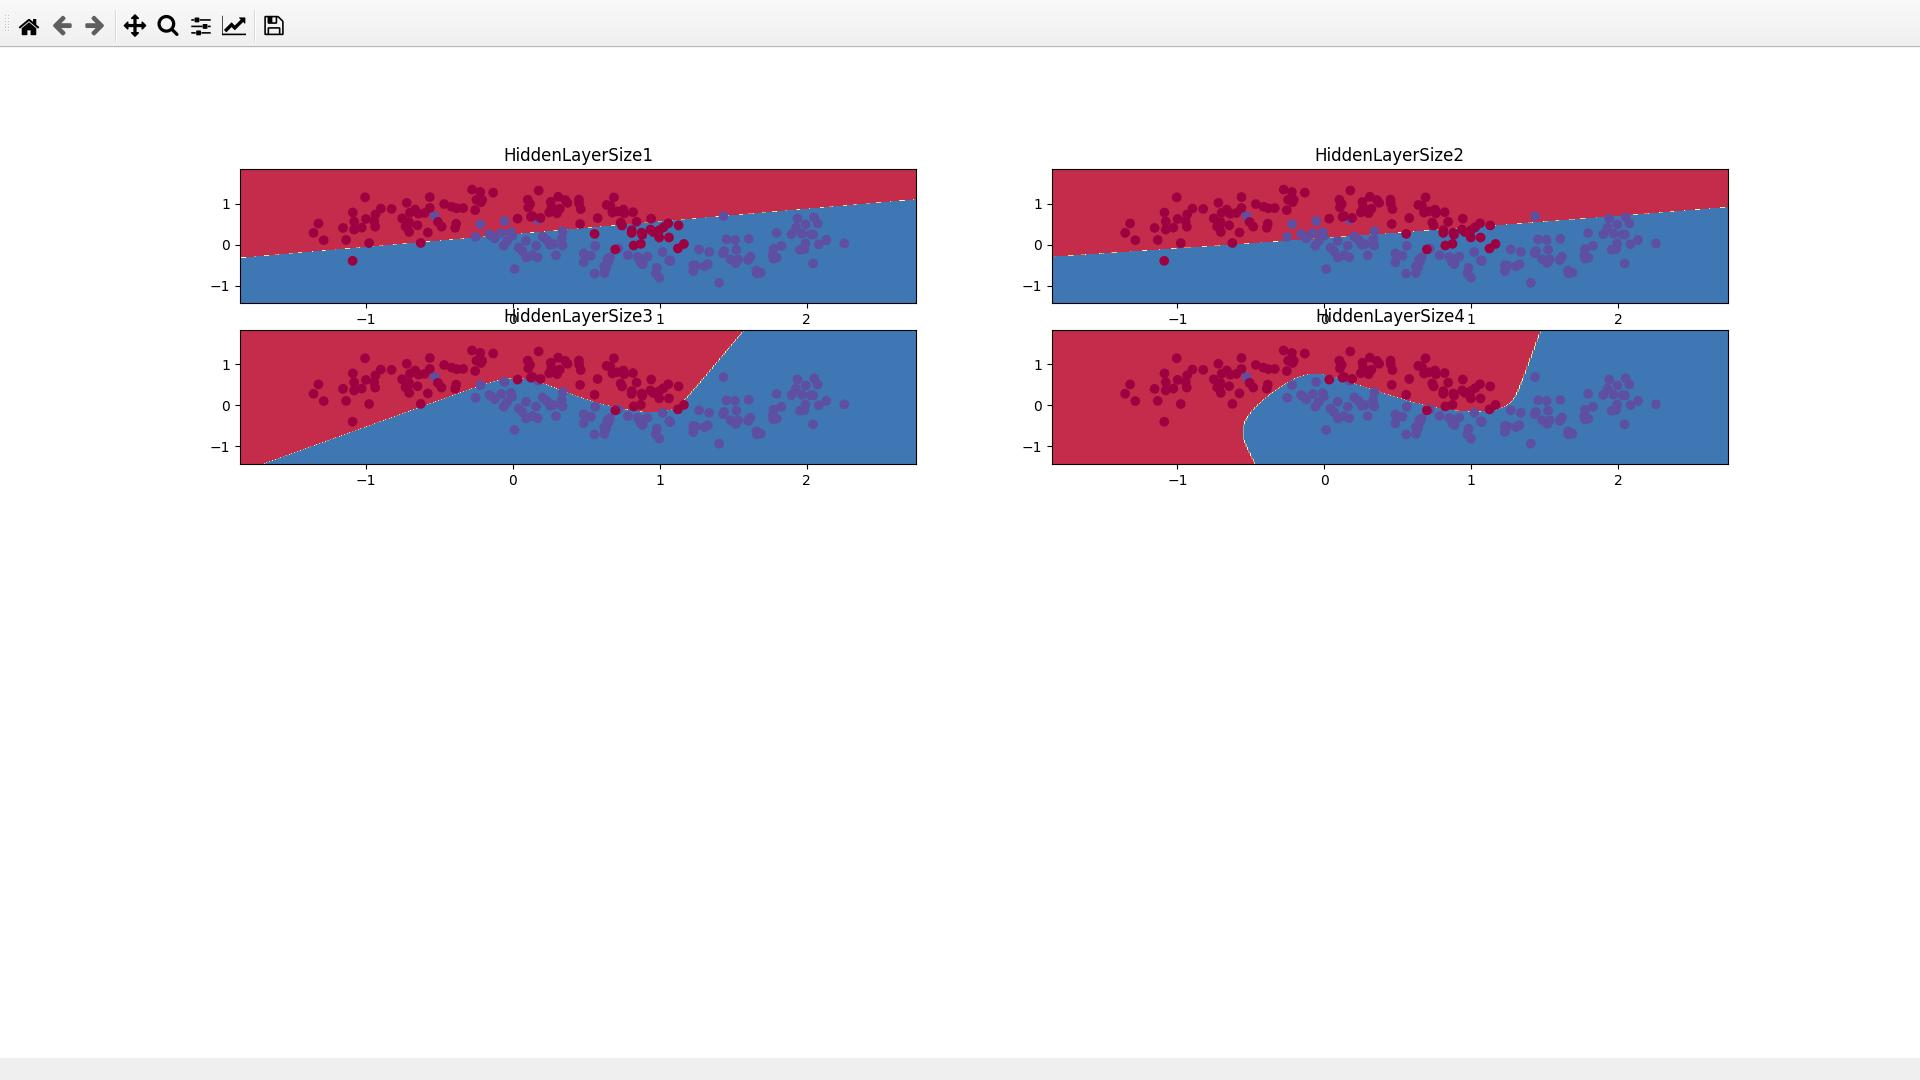
\includegraphics[scale=.25]{plot.jpg}
\end{document}
